\documentclass[11pt]{amsart}
\usepackage[margin=1.15in]{geometry}
\usepackage[T1]{fontenc}
\usepackage{lmodern}
\usepackage{amssymb,amsmath,mathtools}
\usepackage{graphicx,float}
\usepackage[hidelinks]{hyperref}
\usepackage[expansion=false]{microtype}

\newtheorem{theorem}{Theorem}[section]
\newtheorem{proposition}[theorem]{Proposition}
\newtheorem{lemma}[theorem]{Lemma}
\newtheorem{corollary}[theorem]{Corollary}
\newtheorem{mainthm}{Theorem}
\renewcommand{\themainthm}{\Alph{mainthm}}
\theoremstyle{definition}
\newtheorem{definition}[theorem]{Definition}
\newtheorem{remark}[theorem]{Remark}

\newcommand{\RR}{\mathbb{R}}
\newcommand{\Sph}{\mathbb{S}}
\newcommand{\dd}{\,\mathrm{d}}
\newcommand{\jb}[1]{\langle #1\rangle}
\newcommand{\nb}{\|b\|}
\newcommand{\nbi}{\|b\|_\infty}
\newcommand{\hB}{h_{\mathrm B}}
\newcommand{\hL}{h_{\mathrm L}}

\setlength{\emergencystretch}{2.5em}
\hbadness=2000
\raggedbottom
\begin{document}

\title[Only Maxwell molecules contract $W_2$]{Only Maxwell Molecules Contract the Wasserstein Distance Among Power-Law Boltzmann Kernels with Cutoff}

\author{Deep Bhattacharjee}
\address{Formerly, Electro-Gravitational Space Propulsion Laboratory (EGSPL), Bhubaneswar, Odisha 751030, India}
\address{Formerly, University of Calcutta (Heramba Chandra College), 23/49 Gariahat Road, Golpark, Kolkata 700029, West Bengal, India}
\email{d.bhattacharjee@erl-forschung.de}
\email{itsdeep@live.com}
\email{egspl@proton.me (GitHub-related contact; GitHub account creelie)}
\urladdr{https://orcid.org/0000-0003-0466-750X}

\begin{abstract}
Tanaka's theorem says that two Boltzmann solutions never move apart in the quadratic Wasserstein distance when the molecules are Maxwellian. We prove that this fails for every other power law $|v-v_*|^\gamma$ with angular cutoff, $-3<\gamma\le2$, and for the Landau equation with hard potentials, answering Villani's question for these interactions.

\medskip\noindent\textbf{Keywords:} Boltzmann equation; Wasserstein distance; Landau equation.

\smallskip\noindent\textbf{MSC 2020:} 35Q20 (primary); 82C40, 49Q22, 35Q84.
\end{abstract}

\maketitle

\section{Introduction}\label{sec:intro}

The spatially homogeneous Boltzmann equation
\begin{equation}\label{eq:B}
\partial_t f=Q(f,f),\qquad Q(f,f)(v)=\int_{\RR^3}\int_{\Sph^2}B(v-v_*,\sigma)\big(f(v')f(v'_*)-f(v)f(v_*)\big)\dd\sigma\dd v_*,
\end{equation}
with post-collisional velocities
\begin{equation}\label{eq:sigma}
v'=\frac{v+v_*}{2}+\frac{|v-v_*|}{2}\,\sigma,\qquad v'_*=\frac{v+v_*}{2}-\frac{|v-v_*|}{2}\,\sigma,
\end{equation}
describes a spatially uniform rarefied gas whose velocity distribution at time $t$ is $f(t,v)=f_t(v)$. Collisions conserve mass, momentum and kinetic energy. We consider the power-law kernels
\begin{equation}\label{eq:kernel}
B(z,\sigma)=|z|^\gamma\, b(k\cdot\sigma),\qquad k=\frac{z}{|z|},\qquad -3<\gamma\le 2,\quad \gamma\neq0,
\end{equation}
where $b\ge0$ is measurable, not almost everywhere zero, and satisfies Grad's angular cutoff\footnote{Kernels coming from inverse-power forces have $\int b=\infty$, because of grazing collisions; Grad's cutoff removes them. Without the cutoff the gain and loss parts of $Q$ cannot be separated, and the estimates of Sections~\ref{sec:hard} and~\ref{sec:soft} are not available.}
\begin{equation}\label{eq:cutoff}
\nb:=\int_{\Sph^2}b(k\cdot\sigma)\dd\sigma=2\pi\int_{-1}^{1}b(x)\dd x<\infty .
\end{equation}
For $\gamma<0$ we also ask that $b$ be bounded. Hard potentials are $\gamma>0$, hard spheres being $\gamma=1$ with constant $b$; soft potentials are $\gamma<0$. Maxwell molecules, $\gamma=0$, are the excluded case.

For two probability measures $\mu,\nu$ on $\RR^3$ with finite second moments,
\[
W_2(\mu,\nu)^2=\inf_{\pi}\iint|x-y|^2\dd\pi(x,y),
\]
the infimum running over couplings of $\mu$ and $\nu$. Tanaka discovered that for Maxwell molecules $t\mapsto W_2(f_t,g_t)$ is nonincreasing whenever $f$ and $g$ solve \eqref{eq:B} \cite{Tan73,Tan78}, and Toscani and Villani built a uniqueness theory for Maxwell gases on related metrics \cite{TV99}. Tanaka's argument couples the collision histories of the two gases, which is possible because the collision rate of a Maxwell molecule does not depend on the relative speed.

After the proof with Imbert and Silvestre that the Fisher information decreases along \eqref{eq:B} for all physically relevant kernels \cite{ISV25}, which extended the Landau theorem of Guillen and Silvestre \cite{GS25}, Villani asked in the concluding section of his memoir \cite{Vil25} whether $W_2$ enjoys the same robustness: exponential stability is known for various kernels, but could the distance actually be nonincreasing? For the Landau equation with Maxwellian molecules contractivity holds, and for soft potentials a conditional stability estimate is known \cite{CDGT25}; for granular media Carrillo, McCann and Villani proved $W_2$ contraction under uniform convexity \cite{CMV05}.

We answer the question in the negative for all the kernels \eqref{eq:kernel}--\eqref{eq:cutoff}, and for the Landau equation with hard potentials. Fix $e=(0,0,1)$ and a nonnegative even $\eta\in C_c^\infty(\RR^3)$ with $\int\eta=1$ and support in the closed unit ball. For $\delta>0$ and $\rho>0$ let $\eta_\delta(v)=\delta^{-3}\eta(v/\delta)$ and
\begin{equation}\label{eq:data}
j^\delta_\rho(v)=\tfrac12\big(\eta_\delta(v-\rho e)+\eta_\delta(v+\rho e)\big),
\end{equation}
a smooth probability density with zero momentum: two opposite jets of speed $\rho$ and width $\delta$. Given two speeds $r,s>0$ we put $\lambda=s/r$ and use the data
\begin{equation}\label{eq:pairdata}
f_0=j^\delta_r,\qquad g_0=j^{\lambda\delta}_s .
\end{equation}
The second is the image of the first under the dilation $x\mapsto\lambda x$, so the two gases have exactly the same shape and differ only in scale. Define
\begin{equation}\label{eq:J}
\hB(y)=\min\{1,|y-se|,|y+se|\}^8,\qquad J=\int_{\Sph^2}b(e\cdot\sigma)\,\hB(s\sigma)\dd\sigma,\qquad
\Gamma=\frac{2^{\gamma-1}(r^\gamma-s^\gamma)^2J^2}{64\,\lambda\, r^\gamma\,\nb}.
\end{equation}
Since $\hB(s\sigma)>0$ for $\sigma\ne\pm e$ and $b$ is not almost everywhere zero, $J>0$, and $\Gamma>0$ as soon as $r^\gamma\ne s^\gamma$.

\begin{mainthm}\label{thm:A}
Let $B$ satisfy \eqref{eq:kernel}--\eqref{eq:cutoff}, with $b$ bounded if $\gamma<0$. Let $r,s>0$ with $r^\gamma>s^\gamma$, and let $f$ and $g$ be the solutions of \eqref{eq:B} with data \eqref{eq:pairdata}.
\begin{enumerate}
\item[(i)] If $0<\gamma\le2$, there is $t_1>0$ such that for every $t\in(0,t_1]$ there is $\delta_1(t)>0$ with
\[
W_2(f_t,g_t)^2\ \ge\ W_2(f_0,g_0)^2+\tfrac14\,\Gamma\,t\qquad\text{for all }\delta\in(0,\delta_1(t)].
\]
\item[(ii)] If $-3<\gamma<0$, there are $\theta>0$ and $\delta_1>0$ such that for every $\delta\in(0,\delta_1]$ the same inequality holds at the time $t=\theta\,\delta^{2|\gamma|}$.
\end{enumerate}
\end{mainthm}

The condition $r^\gamma>s^\gamma$ means $r>s$ for hard potentials and $r<s$ for soft ones: the gas $g$ is always the one whose jets are destroyed more slowly. For the Landau equation
\begin{equation}\label{eq:L}
\begin{gathered}\partial_tf=Q_L(f,f),\qquad Q_L(f,f)=\nabla_v\cdot\int_{\RR^3}a(v-v_*)\big(f_*\nabla f-f\,\nabla_*f_*\big)\dd v_*,\\ a(z)=|z|^{\gamma+2}\Big(I-\frac{z\otimes z}{|z|^2}\Big),\end{gathered}
\end{equation}
with $f_*=f(v_*)$, put $\vartheta(\tau)=\tau/(1+\tau)$, $\theta_0=\vartheta(4s^2)$ and
\begin{equation}\label{eq:hL}
\hL(y)=\vartheta(|y-se|^2)\,\vartheta(|y+se|^2),\qquad
\Gamma_L=8\,\varepsilon_L\theta_0 s^2\,2^\gamma\Big(\frac{r^\gamma}{1+\varepsilon_L\lambda\theta_0}-s^\gamma\Big),
\end{equation}
where $\varepsilon_L=\min\{(\lambda\|D^2\hL\|_\infty)^{-1},\ ((r/s)^\gamma-1)/(2\lambda\theta_0)\}$. For $r>s$ and $\gamma>0$ one checks that $\Gamma_L>0$ (Section~\ref{sec:landau}).

\begin{mainthm}\label{thm:B}
Let $0<\gamma\le1$ and $r>s>0$, and let $f,g$ be weak solutions of \eqref{eq:L} in the sense of Desvillettes and Villani \cite{DV00} with data \eqref{eq:pairdata}. There is $t_1>0$ such that for every $t\in(0,t_1]$ there is $\delta_1(t)>0$ with $W_2(f_t,g_t)^2\ge W_2(f_0,g_0)^2+\frac14\Gamma_L\,t$ for all $\delta\in(0,\delta_1(t)]$.
\end{mainthm}

\begin{corollary}\label{cor:no}
For every kernel \eqref{eq:kernel}--\eqref{eq:cutoff} with $\gamma\ne0$ (with $b$ bounded if $\gamma<0$), and for the Landau equation with $0<\gamma\le1$, there are two smooth, compactly supported initial data with the same mass and momentum whose solutions satisfy $W_2(f_t,g_t)>W_2(f_0,g_0)$ for some $t>0$. Within the power laws $-3<\gamma\le2$ with cutoff (and $b$ bounded when $\gamma<0$), the map $t\mapsto W_2(f_t,g_t)$ is nonincreasing for all pairs of solutions exactly when $\gamma=0$.
\end{corollary}

The mechanism is a clock mismatch. A pair of opposite jets of speed $\rho$ collides head-on at relative speed $2\rho$, and each such collision sends the two particles to opposite points $\pm\rho\sigma$ of the sphere of radius $\rho$ (Figure~\ref{fig:jets}). The two gases \eqref{eq:pairdata} have the same geometry, but the jets of speed $\rho$ are destroyed at a rate proportional to $\rho^\gamma$ (Figure~\ref{fig:rates}). At time zero the dilation $x\mapsto\lambda x$ is an optimal transport between them. A moment later one gas has spread more of its mass over its sphere than the other, and the dilation is no longer optimal: part of the surplus must be carried back to the poles. In the language of scaling (Remark~\ref{rem:maxwell}), $g_t$ is the dilation of $f_{\lambda^\gamma t}$, and only for $\gamma=0$ do the two clocks agree.

\begin{figure}[H]
\centering
\includegraphics[width=0.86\textwidth]{fig_jets.png}
\caption{The two gases shortly after time zero, drawn for hard potentials ($r>s$). Head-on collisions move mass from the jets $\pm re$ and $\pm se$ to the spheres of radii $r$ and $s$, at rates proportional to $r^\gamma$ and $s^\gamma$. The dots indicate the mass that has left the jets.}\label{fig:jets}
\end{figure}

\begin{figure}[H]
\centering
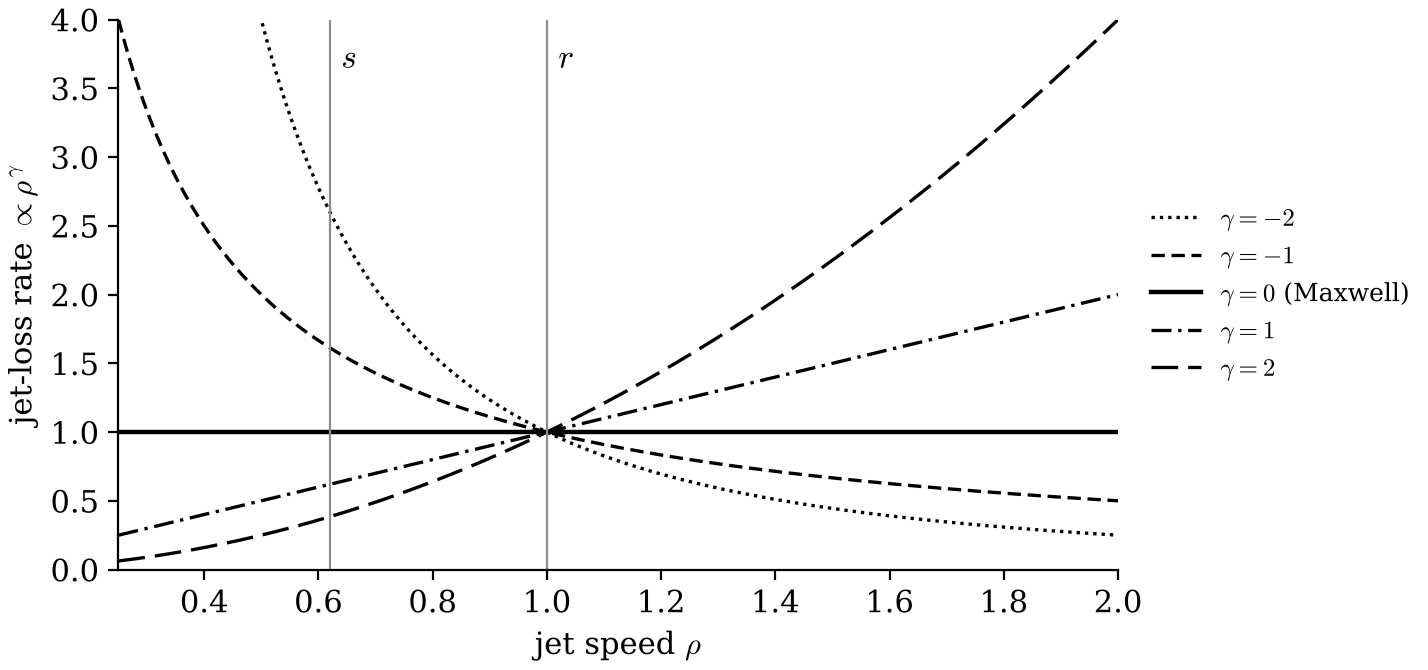
\includegraphics[width=0.82\textwidth]{fig_rates.png}
\caption{Jet-loss rates $\rho^\gamma$. For $\gamma>0$ the faster jets $\pm re$ break up first; for $\gamma<0$ the slower jets $\pm se$ do. Only for Maxwell molecules are the rates equal, and only then does the dilation remain an optimal transport.}\label{fig:rates}
\end{figure}

The proof uses Kantorovich duality in its elementary direction\footnote{If $\varphi(x)+\psi(y)\le|x-y|^2$ for all $x,y$, then integrating against any coupling $\pi$ of $\mu$ and $\nu$ gives $\iint|x-y|^2\dd\pi\ge\int\varphi\dd\mu+\int\psi\dd\nu$. No existence of optimal maps or potentials is needed.}: any pair with $\varphi(x)+\psi(y)\le|x-y|^2$ gives $W_2(\mu,\nu)^2\ge\int\varphi\dd\mu+\int\psi\dd\nu$. We perturb the dilation potentials so as to reward the slower gas for keeping its mass at the poles (Section~\ref{sec:dual}, Figure~\ref{fig:cert}), compute the first variation of the reward exactly in the limit of thin jets (Section~\ref{sec:weak}), and control the error by a short-time expansion. For hard potentials the error is controlled by moments (Section~\ref{sec:hard}). For soft potentials the collision rate inside a jet of width $\delta$ is of order $\delta^\gamma$, which is large; we prove a local theory in norms adapted to the width (Appendix~\ref{app:soft}) and let the time shrink with $\delta$ (Section~\ref{sec:soft}). For the Landau equation collisions are grazing and the first variation sees only second derivatives at the jets, so the certificate must be smooth and curved at the poles (Section~\ref{sec:landau}, Appendix~\ref{app:smooth}).

\section{Weak form and the thin-jet limit}\label{sec:weak}

Write $\jb{v}=(1+|v|^2)^{1/2}$ and $M_k(f)=\int\jb{v}^kf\dd v$. For a bounded continuous $\varphi$ and $v\ne v_*$ set
\begin{equation}\label{eq:Lphi}
L_\varphi(v,v_*)=|v-v_*|^\gamma\int_{\Sph^2}b(k\cdot\sigma)\big(\varphi(v')+\varphi(v'_*)-\varphi(v)-\varphi(v_*)\big)\dd\sigma,\qquad k=\frac{v-v_*}{|v-v_*|},
\end{equation}
with $L_\varphi(v,v)=0$, and for a finite nonnegative measure $\mu$ for which the integral converges absolutely,
\begin{equation}\label{eq:Lambda}
\Lambda_\varphi(\mu)=\frac12\iint L_\varphi(v,v_*)\dd\mu(v)\dd\mu(v_*).
\end{equation}
When $\mu=f\dd v$ and $\iint|v-v_*|^\gamma f f_*<\infty$, the involution $(v,v_*,\sigma)\mapsto(v',v'_*,k)$, which has unit Jacobian and preserves $B$, gives the weak form $\int\varphi\,Q(f,f)\dd v=\Lambda_\varphi(f)$ \cite[Chap.~1]{Vil02}.

\emph{Symmetrisation.} Under $\sigma\mapsto-\sigma$ the velocities $v',v'_*$ are exchanged and $k\cdot\sigma$ changes sign. Hence $Q(f,f)$, $L_\varphi$ and $\nb$ do not change if $b(x)$ is replaced by $(b(x)+b(-x))\mathbf 1_{x\ge0}$, and neither does $J$, because $\hB(s\sigma)$ is even in $\sigma$. We assume from now on that $b$ vanishes on $[-1,0)$; this at most doubles $\nbi$.

\begin{lemma}\label{lem:cont}
For bounded continuous $\varphi$, the function $L_\varphi$ is continuous on $\{v\ne v_*\}$ and $|L_\varphi(v,v_*)|\le4\|\varphi\|_\infty\nb|v-v_*|^\gamma$. If $\gamma>0$, then $L_\varphi$ is continuous on $\RR^3\times\RR^3$ and $|L_\varphi(v,v_*)|\le4\|\varphi\|_\infty\nb\jb{v}^\gamma\jb{v_*}^\gamma$.
\end{lemma}

\begin{proof}
The bracket in \eqref{eq:Lphi} is at most $4\|\varphi\|_\infty$. For $\gamma>0$ the first bound shows continuity on the diagonal, where $L_\varphi$ vanishes, and $|v-v_*|\le\jb{v}\jb{v_*}$ because $2|v||v_*|\le1+|v|^2|v_*|^2$. Let $(v_n,v_{*n})\to(v,v_*)$ with $v\ne v_*$, with unit vectors $k_n\to k$, and choose rotations $R_n\to I$ with $R_nk=k_n$. The substitution $\sigma=R_n\omega$ turns the integral at $(v_n,v_{*n})$ into $\int b(k\cdot\omega)\Psi_n(R_n\omega)\dd\omega$, where $\Psi_n(\sigma)$ is the bracket at $(v_n,v_{*n},\sigma)$. These are bounded by $4\|\varphi\|_\infty$ and converge pointwise to the bracket at $(v,v_*,\omega)$, so dominated convergence applies.
\end{proof}

For $\gamma<0$ we measure concentration by
\begin{equation}\label{eq:S}
S_\gamma(f)=\sup_{v\in\RR^3}\int|f(w)|\,|v-w|^\gamma\dd w\ \le\ C_\gamma\,\delta^\gamma\big(\|f\|_{L^1}+\delta^3\|f\|_\infty\big),\qquad C_\gamma=\frac{4\pi}{\gamma+3},
\end{equation}
valid for every $\delta\in(0,1]$: split the integral at $|v-w|=\delta$ and use $\int_{|u|<\delta}|u|^\gamma\dd u=C_\gamma\delta^{\gamma+3}$ and $C_\gamma\ge1$.

For an even bounded continuous $\varphi$ and $\rho>0$ we define the \emph{thin-jet rate}
\begin{equation}\label{eq:Lstar}
\Lambda^\star_\varphi(\rho)=2^{\gamma-1}\rho^\gamma\int_{\Sph^2}b(e\cdot\sigma)\big(\varphi(\rho\sigma)-\varphi(\rho e)\big)\dd\sigma .
\end{equation}

\begin{lemma}\label{lem:dirac}
Let $\varphi$ be even, bounded and continuous, $\rho>0$ and $\kappa>0$. Then
\[
\Lambda_\varphi(j^{\kappa\delta}_\rho)=\Lambda^\star_\varphi(\rho)+\mathcal E_\delta,\qquad \lim_{\delta\to0}\mathcal E_\delta=0\quad\text{if }\gamma>0 .
\]
If $\gamma<0$ and $|\varphi|\le A_\delta$ on the ball of radius $2\kappa\delta$ about $\rho e$, then $\limsup_{\delta\to0}\big(|\mathcal E_\delta|-4\nb C_\gamma(1+\|\eta\|_\infty)(\kappa\delta)^\gamma A_\delta\big)\le0$.
\end{lemma}

\begin{proof}
Write $\eta^\pm(v)=\eta_{\kappa\delta}(v\mp\rho e)$, so $j^{\kappa\delta}_\rho=\frac12(\eta^++\eta^-)$. By bilinearity and the symmetry $L_\varphi(v,v_*)=L_\varphi(v_*,v)$,
\begin{equation}\label{eq:split}
\Lambda_\varphi(j^{\kappa\delta}_\rho)=\frac18\Big(\iint L_\varphi\,\eta^+\eta^+_*+\iint L_\varphi\,\eta^-\eta^-_*\Big)+\frac14\iint L_\varphi(v,v_*)\,\eta^+(v)\eta^-(v_*)\dd v\dd v_* .
\end{equation}
For $\kappa\delta<\rho$ the support of $\eta^+\otimes\eta^-$ lies in the ball of radius $2\kappa\delta$ about $(\rho e,-\rho e)$, away from the diagonal, so by Lemma~\ref{lem:cont} the last term tends to $\frac14L_\varphi(\rho e,-\rho e)$. At $(v,v_*)=(\rho e,-\rho e)$ we have $k=e$, $v'=\rho\sigma$, $v'_*=-\rho\sigma$, and evenness gives $\frac14L_\varphi(\rho e,-\rho e)=\frac14(2\rho)^\gamma\int b(e\cdot\sigma)\,2(\varphi(\rho\sigma)-\varphi(\rho e))\dd\sigma=\Lambda^\star_\varphi(\rho)$.

If $\gamma>0$, $L_\varphi$ is continuous and vanishes on the diagonal, and $\eta^\pm\otimes\eta^\pm$ converge weakly to $\delta_{(\pm\rho e,\pm\rho e)}$ with supports in a fixed compact set, so the self-terms tend to zero.

Let $\gamma<0$. If $v,v_*$ lie in the ball $B$ of radius $R=\kappa\delta$ about $p=\rho e$ and $w=\frac{v+v_*}2$, then
\[
|v'-p|\le|w-p|+\tfrac12|v-v_*|\le\sqrt2\Big(|w-p|^2+\tfrac14|v-v_*|^2\Big)^{1/2}=\Big(|v-p|^2+|v_*-p|^2\Big)^{1/2}\le\sqrt2R,
\]
by the parallelogram identity, and the same holds for $v'_*$. So the bracket in \eqref{eq:Lphi} is at most $4A_\delta$ on $B\times B$, and by \eqref{eq:S} with $\|\eta^+\|_{L^1}=1$, $(\kappa\delta)^3\|\eta^+\|_\infty=\|\eta\|_\infty$,
\[
\Big|\iint L_\varphi\,\eta^+\eta^+_*\Big|\le4\nb A_\delta\iint\eta^+\eta^+_*|v-v_*|^\gamma\le4\nb A_\delta\, C_\gamma(\kappa\delta)^\gamma(1+\|\eta\|_\infty).
\]
The term with $\eta^-$ is the same by evenness, and the two self-terms carry the weight $\frac18$ each.
\end{proof}

\section{The dual certificate}\label{sec:dual}

Let $r,s>0$ and $\lambda=s/r$. The dilation $x\mapsto\lambda x$ is the gradient of the convex function $\frac\lambda2|x|^2$, and its Kantorovich potentials for the cost $|x-y|^2$ are
\begin{equation}\label{eq:pot0}
\varphi_0(x)=(1-\lambda)|x|^2,\qquad \psi_0(y)=\Big(1-\frac1\lambda\Big)|y|^2,\qquad |x-y|^2-\psi_0(y)=\frac1\lambda|y-\lambda x|^2+\varphi_0(x),
\end{equation}
the identity being a completion of the square. Let $h\ge0$ be bounded and continuous, and for $\varepsilon>0$ put
\begin{equation}\label{eq:pair}
\begin{gathered}\psi_\varepsilon=\psi_0-\varepsilon h,\qquad \varphi_\varepsilon(x)=\inf_{y}\big(|x-y|^2-\psi_\varepsilon(y)\big)=\varphi_0(x)+m_\varepsilon(\lambda x),\\ m_\varepsilon(z)=\inf_y\Big(\frac1\lambda|y-z|^2+\varepsilon h(y)\Big).\end{gathered}
\end{equation}
By construction\footnote{$\varphi_\varepsilon$ is the $c$-transform of $\psi_\varepsilon$; the inequality $\varphi_\varepsilon(x)+\psi_\varepsilon(y)\le|x-y|^2$ is its definition read backwards.} $\varphi_\varepsilon(x)+\psi_\varepsilon(y)\le|x-y|^2$. We write
\begin{equation}\label{eq:tilde}
\tilde\varphi_\varepsilon(x)=m_\varepsilon(\lambda x),\qquad\tilde\psi_\varepsilon=-\varepsilon h .
\end{equation}

\begin{lemma}\label{lem:m}
$m_\varepsilon$ is continuous, $0\le m_\varepsilon\le\varepsilon h$, and $m_\varepsilon$ is even if $h$ is. If $h$ is $\ell$-Lipschitz, then $m_\varepsilon\ge\varepsilon h-\frac14\lambda\ell^2\varepsilon^2$.
\end{lemma}

\begin{proof}
The upper bound is the choice $y=z$. The infimum may be restricted to $|y-z|\le(\lambda\varepsilon\|h\|_\infty)^{1/2}$, where the functions $z\mapsto\frac1\lambda|y-z|^2$ are uniformly Lipschitz, so $m_\varepsilon$ is locally Lipschitz. If $h$ is $\ell$-Lipschitz then, with $u=|y-z|$, $\frac1\lambda u^2+\varepsilon h(y)\ge\varepsilon h(z)+\frac1\lambda u^2-\varepsilon\ell u\ge\varepsilon h(z)-\frac14\lambda\ell^2\varepsilon^2$.
\end{proof}

\begin{proposition}\label{prop:master}
Let $f,g$ be solutions (of \eqref{eq:B} or of \eqref{eq:L}) with data \eqref{eq:pairdata} that conserve mass and energy. Then $W_2(f_0,g_0)^2=(1-\lambda)^2(r^2+\delta^2m_2)$, $m_2=\int|w|^2\eta(w)\dd w$, and for every $t\ge0$
\begin{equation}\label{eq:master}
W_2(f_t,g_t)^2-W_2(f_0,g_0)^2\ \ge\ \Big(\int\tilde\varphi_\varepsilon f_t-\int\tilde\varphi_\varepsilon f_0\Big)+\Big(\int\tilde\psi_\varepsilon g_t-\int\tilde\psi_\varepsilon g_0\Big)-\varepsilon\int h\,g_0 .
\end{equation}
\end{proposition}

\begin{proof}
Let $E=\int|v|^2f_0=r^2+\delta^2m_2$ (the cross term vanishes because $\eta$ is even). Since $g_0$ is the image of $f_0$ under $x\mapsto\lambda x$, $\int|v|^2g_0=\lambda^2E$, and the dilation coupling gives $W_2(f_0,g_0)^2\le(1-\lambda)^2E$. Conversely, \eqref{eq:pot0} and duality give $W_2(f_0,g_0)^2\ge(1-\lambda)E+(1-\lambda^{-1})\lambda^2E=(1-\lambda)^2E$. At time $t$, by duality with $(\varphi_\varepsilon,\psi_\varepsilon)$ and conservation of energy,
\[
W_2(f_t,g_t)^2\ge(1-\lambda)E+\Big(1-\frac1\lambda\Big)\lambda^2E+\int\tilde\varphi_\varepsilon f_t+\int\tilde\psi_\varepsilon g_t .
\]
The first two terms equal $W_2(f_0,g_0)^2$. Finally $\int\tilde\varphi_\varepsilon f_0\ge0$ and $\int\tilde\psi_\varepsilon g_0=-\varepsilon\int hg_0$.
\end{proof}

For the Boltzmann equation we take $h=\hB$ from \eqref{eq:J}. It is even, takes values in $[0,1]$, is $8$-Lipschitz, vanishes exactly at $\pm se$, and $\hB(y)\le|y\mp se|^8$. Since $g_0$ is supported within $\lambda\delta$ of $\pm se$,
\begin{equation}\label{eq:deficitB}
\varepsilon\int\hB\, g_0\le\varepsilon(\lambda\delta)^8 .
\end{equation}

\begin{proposition}\label{prop:gain}
With $h=\hB$, the thin-jet gain $\Gamma_\varepsilon:=\Lambda^\star_{\tilde\varphi_\varepsilon}(r)+\Lambda^\star_{\tilde\psi_\varepsilon}(s)$ satisfies
\[
\Gamma_\varepsilon\ \ge\ 2^{\gamma-1}\Big(\varepsilon\,(r^\gamma-s^\gamma)\,J-16\,\varepsilon^2\lambda\, r^\gamma\nb\Big),
\]
and for $\varepsilon_*=(r^\gamma-s^\gamma)J/(32\lambda r^\gamma\nb)$ the right-hand side equals $\Gamma$ of \eqref{eq:J}.
\end{proposition}

\begin{proof}
On the sphere of radius $r$, $\tilde\varphi_\varepsilon(r\sigma)=m_\varepsilon(s\sigma)$ and $\tilde\varphi_\varepsilon(re)=m_\varepsilon(se)=0$; on the sphere of radius $s$, $\tilde\psi_\varepsilon(s\sigma)=-\varepsilon\hB(s\sigma)$ and $\tilde\psi_\varepsilon(se)=0$. Thus
\[
\Gamma_\varepsilon=2^{\gamma-1}\Big(r^\gamma\int b(e\cdot\sigma)\,m_\varepsilon(s\sigma)\dd\sigma-\varepsilon s^\gamma J\Big),
\]
and Lemma~\ref{lem:m} with $\ell=8$ gives $\int b(e\cdot\sigma)m_\varepsilon(s\sigma)\dd\sigma\ge\varepsilon J-16\lambda\varepsilon^2\nb$. The value at $\varepsilon_*$ is a direct computation.
\end{proof}

The gain has a transparent meaning. The term $-\varepsilon s^\gamma J$ is the price paid by the gas $g$ for mass leaving its poles, and $r^\gamma\int b\,m_\varepsilon(s\sigma)$ is the reward collected by $f$ for mass reaching its sphere; up to $O(\varepsilon^2)$ the reward and the price are the same integral with the two clocks $r^\gamma$ and $s^\gamma$ (Figure~\ref{fig:cert}).

\begin{figure}[H]
\centering
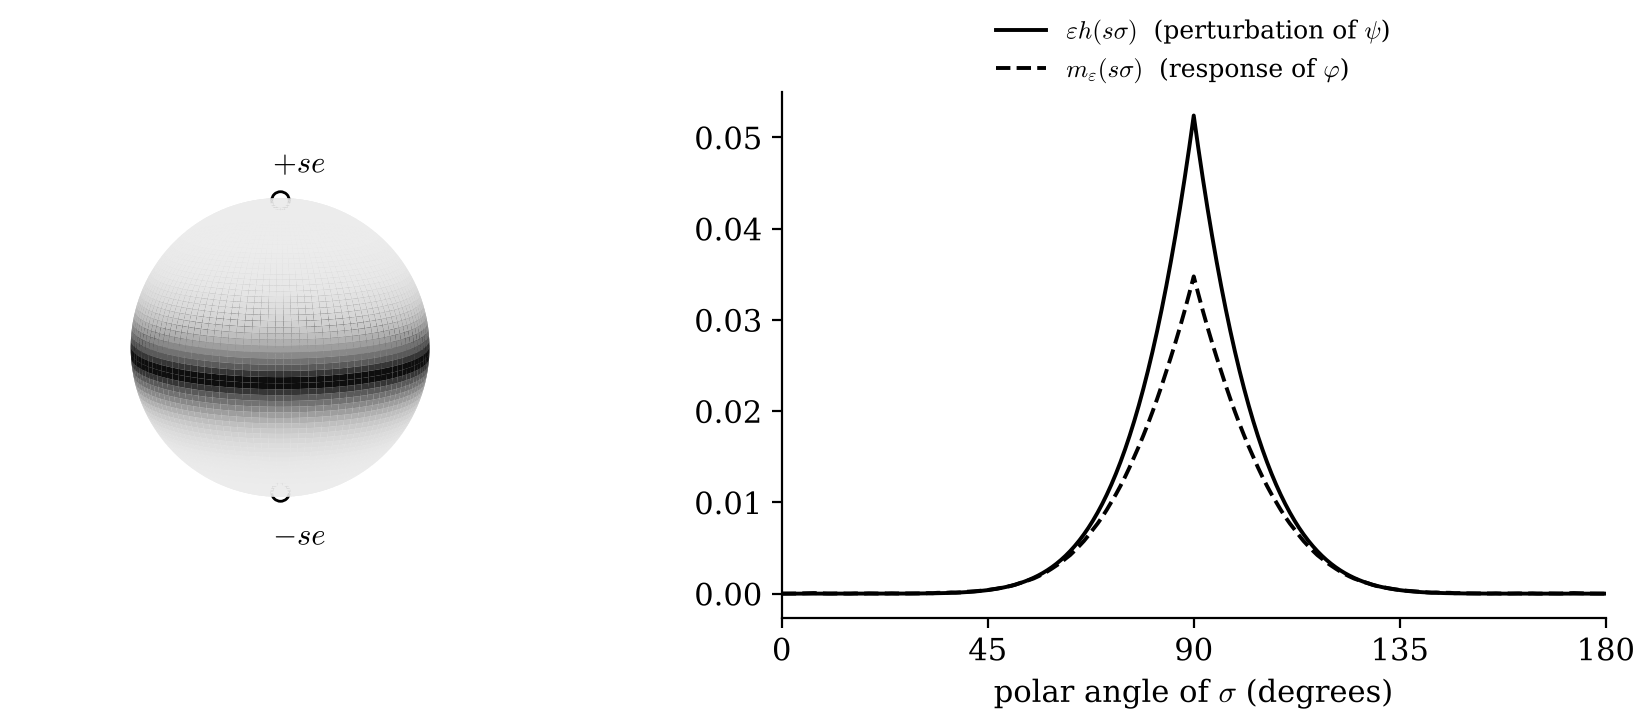
\includegraphics[width=0.95\textwidth]{fig_certificate.png}
\caption{The certificate on the sphere of radius $s$ (shaded by $\hB$, white at the poles) and its profile along a meridian, for $\lambda=0.62$ and $\varepsilon=0.15$. The perturbation $\varepsilon\hB$ of $\psi$ is answered by the smaller but comparable bump $m_\varepsilon$ in $\varphi$; both vanish to eighth order at the poles, where the jets sit.}\label{fig:cert}
\end{figure}

\section{Hard potentials}\label{sec:hard}

Let $0<\gamma\le2$. We use the $L^1$ theory of \eqref{eq:B} for hard potentials with cutoff, due to Arkeryd, Elmroth, Desvillettes, Wennberg, and Mischler and Wennberg \cite{MW99,Wen97}: for every nonnegative $f_0$ with $M_2(f_0)<\infty$ there is a unique solution $f\in C([0,\infty);L^1_2)$ that conserves mass, momentum and energy and satisfies $f_t=f_0+\int_0^tQ(f_\tau,f_\tau)\dd\tau$, and every moment finite at time zero stays bounded on bounded time intervals \cite[Sect.~1]{MW99}. The data \eqref{eq:pairdata} have compact support.

\begin{lemma}\label{lem:moments}
Let $K_0\ge M_4(f_0)$ and $T=(2\nb K_0)^{-1}$. Then $M_4(f_t)\le2K_0$ for $0\le t\le T$.
\end{lemma}

\begin{proof}
By the weak form with $\varphi=\jb{v}^4$ (legitimate because $M_6$ is locally bounded),
\[
\frac{\dd}{\dd t}M_4(f_t)=\frac12\iint ff_*|v-v_*|^\gamma\int b(k\cdot\sigma)\big(\jb{v'}^4+\jb{v'_*}^4-\jb{v}^4-\jb{v_*}^4\big)\dd\sigma\dd v\dd v_* .
\]
Energy conservation in a collision gives $\jb{v'}^2+\jb{v'_*}^2=\jb{v}^2+\jb{v_*}^2$, so $\jb{v'}^4+\jb{v'_*}^4\le(\jb{v}^2+\jb{v_*}^2)^2$ and the bracket is at most $2\jb{v}^2\jb{v_*}^2$. With $|v-v_*|^\gamma\le\jb{v}^\gamma\jb{v_*}^\gamma$ and $\gamma\le2$, $\frac{\dd}{\dd t}M_4\le\nb M_{2+\gamma}^2\le\nb M_4^2$, and $M_4(f_t)\le K_0/(1-\nb K_0t)\le2K_0$ for $t\le T$.
\end{proof}

\begin{lemma}\label{lem:expansion}
If $M_4(f_\tau)\le K$ for $0\le\tau\le t$, then for every bounded continuous $\varphi$
\[
\Big|\int\varphi f_t-\int\varphi f_0-t\,\Lambda_\varphi(f_0)\Big|\le 8\,\|\varphi\|_\infty\nb^2K^3\,t^2 .
\]
\end{lemma}

\begin{proof}
First, $\|Q(f,f)\|_{L^1_\gamma}\le4\nb M_{2\gamma}(f)M_\gamma(f)$: indeed $\int\jb{v}^\gamma|Q(f,f)|\le\iiint Bff_*(\jb{v'}^\gamma+\jb{v}^\gamma)$ after the involution in the gain term, $\jb{v'}^\gamma\le(\jb{v}^2+\jb{v_*}^2)^{\gamma/2}\le\jb{v}^\gamma+\jb{v_*}^\gamma$ since $\gamma\le2$, and $|v-v_*|^\gamma\le\jb{v}^\gamma\jb{v_*}^\gamma$. Since $M_\gamma\le M_{2\gamma}\le M_4$, $\|f_\tau-f_0\|_{L^1_\gamma}\le4\nb K^2\tau$. By Lemma~\ref{lem:cont} and $|f_\tau f_{\tau*}-f_0f_{0*}|\le|f_\tau-f_0|f_{\tau*}+f_0|f_{\tau*}-f_{0*}|$,
\[
|\Lambda_\varphi(f_\tau)-\Lambda_\varphi(f_0)|\le2\|\varphi\|_\infty\nb\,\|f_\tau-f_0\|_{L^1_\gamma}\big(M_\gamma(f_\tau)+M_\gamma(f_0)\big)\le16\|\varphi\|_\infty\nb^2K^3\tau .
\]
Integrating $\int\varphi f_t-\int\varphi f_0=\int_0^t\Lambda_\varphi(f_\tau)\dd\tau$ over $[0,t]$ gives the claim.
\end{proof}

\begin{proof}[Proof of Theorem~\ref{thm:A}\textup{(i)}]
Here $r>s$, so $\lambda<1$. Fix $\varepsilon=\varepsilon_*$, so that $\Gamma_\varepsilon\ge\Gamma$, and note $\|\tilde\varphi_\varepsilon\|_\infty,\|\tilde\psi_\varepsilon\|_\infty\le\varepsilon$. For $\delta\le1$ both data are supported in the ball of radius $r+1$, so $M_4\le K_0:=(1+(r+1)^2)^2$; with $T=(2\nb K_0)^{-1}$ and $K=2K_0$, Lemma~\ref{lem:moments} bounds $M_4(f_\tau),M_4(g_\tau)$ by $K$ for $\tau\le T$. Proposition~\ref{prop:master}, Lemma~\ref{lem:expansion} and \eqref{eq:deficitB} give, for $t\le T$,
\begin{equation}\label{eq:finalhard}
W_2(f_t,g_t)^2-W_2(f_0,g_0)^2\ \ge\ t\,\Gamma^\delta_\varepsilon-16\,\varepsilon\nb^2K^3t^2-\varepsilon(\lambda\delta)^8,\qquad \Gamma^\delta_\varepsilon=\Lambda_{\tilde\varphi_\varepsilon}(f_0)+\Lambda_{\tilde\psi_\varepsilon}(g_0).
\end{equation}
By Lemma~\ref{lem:dirac} (with $\kappa=1$ and $\kappa=\lambda$), $\Gamma^\delta_\varepsilon\to\Gamma_\varepsilon\ge\Gamma$ as $\delta\to0$. Let $t_1=\min\{T,\Gamma/(64\varepsilon\nb^2K^3)\}$ and $0<t\le t_1$, so that $16\varepsilon\nb^2K^3t^2\le\frac14t\Gamma$, and choose $\delta_1(t)$ such that $\Gamma^\delta_\varepsilon\ge\frac34\Gamma$ and $\varepsilon(\lambda\delta)^8\le\frac14t\Gamma$ for $\delta\le\delta_1(t)$. The right-hand side of \eqref{eq:finalhard} is then at least $t\Gamma(\frac34-\frac14-\frac14)=\frac14t\Gamma$.
\end{proof}

\section{Soft potentials}\label{sec:soft}

Let $-3<\gamma<0$ and $b$ bounded (and supported in $k\cdot\sigma\ge0$). For $0<\delta\le1$ we use the norm
\begin{equation}\label{eq:norm}
\|f\|_\delta=\int\jb{v}^2|f(v)|\dd v+\delta^3\|f\|_\infty ,
\end{equation}
which gives the same weight to a jet of width $\delta$ and unit mass whatever $\delta$ is. By \eqref{eq:S}, $S_\gamma(f)\le C_\gamma\delta^\gamma\|f\|_\delta$. The following local theory is proved in Appendix~\ref{app:soft}.

\begin{proposition}\label{prop:local}
Let $f_0\ge0$ with $N\ge\|f_0\|_\delta$, let $C_1=C_\gamma(2\nb+32\pi\nbi)$ and $T_\delta=\delta^{|\gamma|}/(16C_1N)$. There is a unique nonnegative solution $f\in C([0,T_\delta];L^1_2\cap L^\infty)$ of $f_t=f_0+\int_0^tQ(f_\tau,f_\tau)\dd\tau$. It conserves mass, momentum and energy, and $\|f_t\|_\delta\le2N$ for $0\le t\le T_\delta$.
\end{proposition}

\begin{lemma}\label{lem:expsoft}
In the setting of Proposition~\ref{prop:local} with $\int f_0=1$, for every bounded continuous $\varphi$ and $0\le t\le T_\delta$,
\[
\Big|\int\varphi f_t-\int\varphi f_0-t\,\Lambda_\varphi(f_0)\Big|\le 24\,C_\gamma^2\nb^2N^3\,\|\varphi\|_\infty\,\delta^{2\gamma}\,t^2 .
\]
\end{lemma}

\begin{proof}
The weak form holds because $\iiint B ff_*\le\nb\|f\|_{L^1}S_\gamma(f)<\infty$, and the same bound gives $\|Q(f,f)\|_{L^1}\le2\nb\|f\|_{L^1}S_\gamma(f)$, with the involution in the gain term. For $\tau\le T_\delta$, $\|f_\tau\|_{L^1}=1$ and $S_\gamma(f_\tau)\le2C_\gamma\delta^\gamma N$, so $\|f_\tau-f_0\|_{L^1}\le4\nb C_\gamma\delta^\gamma N\tau$. By Lemma~\ref{lem:cont},
\[
|\Lambda_\varphi(f_\tau)-\Lambda_\varphi(f_0)|\le2\|\varphi\|_\infty\nb\,\|f_\tau-f_0\|_{L^1}\big(S_\gamma(f_\tau)+S_\gamma(f_0)\big)\le24\,C_\gamma^2\nb^2N^2\|\varphi\|_\infty\delta^{2\gamma}\tau,
\]
and integration over $[0,t]$, with $N\ge1$, gives the claim.
\end{proof}

\begin{proof}[Proof of Theorem~\ref{thm:A}\textup{(ii)}]
Here $r<s$, so $\lambda>1$. For $\delta\le\min\{1,r/2\}$ the jets of $f_0$ and of $g_0$ are disjoint and
\[
\|f_0\|_\delta,\ \|g_0\|_\delta\ \le\ N:=1+(s+\lambda)^2+\lambda^{-3}\|\eta\|_\infty+\|\eta\|_\infty+1,
\]
because $\delta^3\|j^{\kappa\delta}_\rho\|_\infty\le\kappa^{-3}\|\eta\|_\infty$ and both data are supported in the ball of radius $s+\lambda$. Fix $\varepsilon=\varepsilon_*$ and let $C_3=48C_\gamma^2\nb^2N^3$. Proposition~\ref{prop:master}, Lemma~\ref{lem:expsoft} for $\tilde\varphi_\varepsilon$ and $\tilde\psi_\varepsilon$, and \eqref{eq:deficitB} give, for $t\le T_\delta$,
\begin{equation}\label{eq:finalsoft}
W_2(f_t,g_t)^2-W_2(f_0,g_0)^2\ \ge\ t\,\Gamma^\delta_\varepsilon-\varepsilon C_3\,\delta^{2\gamma}t^2-\varepsilon(\lambda\delta)^8 .
\end{equation}

\emph{The gain.} On the ball of radius $2\delta$ about $\pm re$, $|\tilde\varphi_\varepsilon(x)|\le\varepsilon\hB(\lambda x)\le\varepsilon|\lambda x\mp se|^8\le\varepsilon\lambda^8(2\delta)^8$, and on the ball of radius $2\lambda\delta$ about $\pm se$, $|\tilde\psi_\varepsilon|\le\varepsilon(2\lambda\delta)^8$. Lemma~\ref{lem:dirac} (with $\kappa=1$ and $\kappa=\lambda$) therefore gives $|\Gamma^\delta_\varepsilon-\Gamma_\varepsilon|\le o(1)+C\varepsilon\delta^{8+\gamma}$ as $\delta\to0$, so $\Gamma^\delta_\varepsilon\to\Gamma_\varepsilon\ge\Gamma$. The decay $\delta^{8+\gamma}$ is where the eighth-order vanishing of $\hB$ at the poles is used: collisions of two particles of the same jet are frequent, at rate $\delta^\gamma$, but they do not move the particles off the jet, where the certificate is flat.

\emph{Choice of the time.} Put $t=\theta\delta^{2|\gamma|}$ with
\[
\theta=\min\Big\{\frac{1}{16C_1N},\ \frac{\Gamma}{4\varepsilon C_3}\Big\}.
\]
Since $\delta\le1$, $t\le\delta^{|\gamma|}/(16C_1N)=T_\delta$ (for $f$ and for $g$), and $\varepsilon C_3\delta^{2\gamma}t^2=\varepsilon C_3\theta\,t\le\frac14\Gamma t$. Choose $\delta_1\le\min\{1,r/2\}$ so small that for $\delta\le\delta_1$ we have $\Gamma^\delta_\varepsilon\ge\frac34\Gamma$ and $\varepsilon\lambda^8\delta^{8-2|\gamma|}\le\frac14\theta\Gamma$; the latter is possible because $8-2|\gamma|>2$. Then $\varepsilon(\lambda\delta)^8\le\frac14\Gamma t$, and \eqref{eq:finalsoft} gives $W_2(f_t,g_t)^2-W_2(f_0,g_0)^2\ge\frac14\Gamma t$.
\end{proof}

\section{The Landau equation with hard potentials}\label{sec:landau}

Let $0<\gamma\le1$. With $a$ as in \eqref{eq:L} and $\beta(z)=\nabla\cdot a(z)=-2|z|^\gamma z$, the weak form of \eqref{eq:L} reads \cite[Chap.~1]{Vil02}
\begin{equation}\label{eq:weakL}
\begin{gathered}\int\varphi\,Q_L(f,f)=\frac12\iint ff_*\,K_\varphi(v,v_*),\\
K_\varphi(v,w)=a(v-w):\big(D^2\varphi(v)+D^2\varphi(w)\big)+2\beta(v-w)\cdot\big(\nabla\varphi(v)-\nabla\varphi(w)\big).\end{gathered}
\end{equation}
We write $\Lambda^L_\varphi(\mu)=\frac12\iint K_\varphi\dd\mu\dd\mu$. Desvillettes and Villani \cite{DV00} proved that for $0\le f_0\in L^1$ with finite moments and entropy there is a weak solution of \eqref{eq:L}: it conserves mass, momentum and energy, every moment finite at time zero stays bounded on $[0,1]$ by a constant depending only on that initial moment, and $\int\varphi f_t=\int\varphi f_0+\int_0^t\Lambda^L_\varphi(f_\tau)\dd\tau$ for $C^2$ test functions with bounded second derivatives. By truncation and the moment bounds this identity extends to $C^2$ functions $\varphi$ with $|\varphi(v)|+\|D^2\varphi(v)\|\le A\jb{v}^q$ whenever $M_{q+\gamma+2}$ stays bounded, the right-hand side being dominated through Lemma~\ref{lem:K} below.

\begin{lemma}\label{lem:K}
Let $\varphi\in C^2$. Then $K_\varphi$ is continuous, $K_\varphi(v,v)=0$, and
\[
|K_\varphi(v,w)|\le8\,|v-w|^{\gamma+2}\sup_{u\in[v,w]}\|D^2\varphi(u)\| .
\]
If $\varphi\in C^4$ with bounded derivatives up to order four, then $v\mapsto K_\varphi(v,w)$ is $C^2$ and $\|D_v^2K_\varphi(v,w)\|\le C\|\varphi\|_{C^4}(1+|v-w|)^{\gamma+2}$, with $C$ depending only on $\gamma$.
\end{lemma}

\begin{proof}
Since $a(z)$ is $|z|^{\gamma+2}$ times a projection of rank two, $|a(z):A|\le2|z|^{\gamma+2}\|A\|$. Also $|\beta(z)|=2|z|^{\gamma+1}$ and $|\nabla\varphi(v)-\nabla\varphi(w)|\le|v-w|\sup_{[v,w]}\|D^2\varphi\|$. This gives the bound, continuity and $K_\varphi(v,v)=0$, since $\gamma+2>0$. For the second statement put $z=v-w$ and write $\nabla\varphi(v)-\nabla\varphi(w)=A(v,w)z$ with $A(v,w)=\int_0^1D^2\varphi(w+\tau z)\dd\tau$, which is $C^2$ in $v$. Then $K_\varphi(v,w)=a(z):(D^2\varphi(v)+D^2\varphi(w))-4|z|^\gamma\,z\cdot A(v,w)z$. The functions $a(z)$ and $|z|^\gamma z\otimes z$ are positively homogeneous of degree $\gamma+2>2$ and smooth off the origin, so they are $C^2$ on $\RR^3$ with second derivatives bounded by $C|z|^\gamma$ and first derivatives bounded by $C|z|^{\gamma+1}$. Differentiating the products twice in $v$ and using $\|A\|,\|D_vA\|,\|D_v^2A\|\le\|\varphi\|_{C^4}$ gives the bound.
\end{proof}

\begin{lemma}\label{lem:diracL}
Let $\varphi\in C^2$ be even with bounded second derivatives, $\rho>0$, $\kappa>0$, and write $\Delta_\perp$ for the Laplacian in the plane orthogonal to $e$ and $\partial_e=e\cdot\nabla$. Then
\[
\lim_{\delta\to0}\Lambda^L_\varphi(j^{\kappa\delta}_\rho)=(2\rho)^\gamma\big(2\rho^2\,\Delta_\perp\varphi(\rho e)-4\rho\,\partial_e\varphi(\rho e)\big).
\]
\end{lemma}

\begin{proof}
By Lemma~\ref{lem:K} and weak convergence, the limit is $\frac18\sum K_\varphi(\pm\rho e,\pm\rho e)$ over the four sign pairs. The diagonal terms vanish. At $(\rho e,-\rho e)$, $z=2\rho e$, $a(z)=(2\rho)^{\gamma+2}(I-e\otimes e)$ and $\beta(z)=-2(2\rho)^{\gamma}\,2\rho\,e$. Evenness gives $D^2\varphi(-\rho e)=D^2\varphi(\rho e)$ and $\nabla\varphi(-\rho e)=-\nabla\varphi(\rho e)$, so $K_\varphi(\rho e,-\rho e)=2(2\rho)^{\gamma+2}\Delta_\perp\varphi(\rho e)-16\rho(2\rho)^\gamma\partial_e\varphi(\rho e)$, and the same value at $(-\rho e,\rho e)$. Dividing $2K_\varphi(\rho e,-\rho e)$ by $8$ gives the claim.
\end{proof}

For $\varphi=|v|^2$ the limit is $(2\rho)^\gamma(8\rho^2-8\rho^2)=0$, as energy conservation requires: transverse diffusion and longitudinal friction balance. The certificate has to see the diffusion term, so a function that vanishes to high order at the poles is useless here. This is why \eqref{eq:hL} is curved at $\pm se$: $\hL(\pm se)=0$, $\nabla\hL(\pm se)=0$ and $D^2\hL(\pm se)=2\theta_0 I$. Indeed, near $se$ the first factor is $|y-se|^2+O(|y-se|^4)$, because $\vartheta(0)=0$ and $\vartheta'(0)=1$, while the second factor is smooth and equals $\vartheta(4s^2)=\theta_0$ at $se$; the point $-se$ is symmetric. The function $\hL$ is smooth, even, takes values in $[0,1)$, has bounded derivatives of all orders, and $\hL(y)\le|y\mp se|^2$ because $\vartheta(\tau)\le\min\{\tau,1\}$.

\begin{lemma}\label{lem:smooth}
Let $h\ge0$ be smooth with bounded derivatives of all orders and $0<\varepsilon\le(\lambda\|D^2h\|_\infty)^{-1}$. Then $m_\varepsilon\in C^\infty$ with bounded derivatives of all orders. If $\nabla h(p)=0$, then $m_\varepsilon(p)=\varepsilon h(p)$, $\nabla m_\varepsilon(p)=0$ and $D^2m_\varepsilon(p)=\varepsilon D^2h(p)\big(I+\tfrac{\varepsilon\lambda}2D^2h(p)\big)^{-1}$.
\end{lemma}

The proof is in Appendix~\ref{app:smooth}. For $h=\hL$ and $p=se$ it gives $D^2m_\varepsilon(se)=\frac{2\varepsilon\theta_0}{1+\varepsilon\lambda\theta_0}I$.

\begin{proof}[Proof of Theorem~\ref{thm:B}]
Let $\varepsilon=\varepsilon_L$, $h=\hL$, and $\tilde\varphi=\tilde\varphi_\varepsilon$, $\tilde\psi=\tilde\psi_\varepsilon$; both are even and lie in $C^4$ with bounded derivatives (Lemma~\ref{lem:smooth}). Since $\tilde\varphi(x)=m_\varepsilon(\lambda x)$, $\nabla\tilde\varphi(re)=0$ and $\Delta_\perp\tilde\varphi(re)=\lambda^2\cdot2\cdot\frac{2\varepsilon\theta_0}{1+\varepsilon\lambda\theta_0}$, while $\nabla\tilde\psi(se)=0$ and $\Delta_\perp\tilde\psi(se)=-4\varepsilon\theta_0$. By Lemma~\ref{lem:diracL}, using $\lambda r=s$,
\[
\Lambda^L_{\tilde\varphi}(f_0)+\Lambda^L_{\tilde\psi}(g_0)\ \longrightarrow\ (2r)^\gamma\,\frac{8s^2\varepsilon\theta_0}{1+\varepsilon\lambda\theta_0}-(2s)^\gamma\,8s^2\varepsilon\theta_0=\Gamma_L\qquad(\delta\to0).
\]
Since $\varepsilon\lambda\theta_0\le\frac12((r/s)^\gamma-1)$, we have $r^\gamma/(1+\varepsilon\lambda\theta_0)\ge2r^\gamma s^\gamma/(r^\gamma+s^\gamma)>s^\gamma$, so $\Gamma_L>0$.

\emph{Error.} Let $K$ bound $M_6(f_\tau),M_6(g_\tau)$ for $\tau\le1$ and $\delta\le1$; it exists because $M_6$ of the data is at most $(1+(r+1)^2)^3$. For $\varphi\in\{\tilde\varphi,\tilde\psi\}$ and $\tau\le1$, by symmetry of $K_\varphi$,
\[
\Lambda^L_\varphi(f_\tau)-\Lambda^L_\varphi(f_0)=\frac12\int f_\tau(w)\Big(\int(f_\tau-f_0)\,K_\varphi(\cdot,w)\Big)\dd w+\frac12\int f_0(w)\Big(\int(f_\tau-f_0)\,K_\varphi(\cdot,w)\Big)\dd w .
\]
By Lemma~\ref{lem:K}, $\psi_w=K_\varphi(\cdot,w)$ is $C^2$ with $|\psi_w(u)|+\|D^2\psi_w(u)\|\le C_\varphi\jb{u}^{\gamma+2}\jb{w}^{\gamma+2}$, so the weak formulation applies and $\int(f_\tau-f_0)\psi_w=\int_0^\tau\Lambda^L_{\psi_w}(f_u)\dd u$. The first bound of Lemma~\ref{lem:K}, applied to $\psi_w$, together with $\sup_{u\in[v,v_*]}\jb{u}^{\gamma+2}\le2^{\gamma+2}\jb{v}^{\gamma+2}\jb{v_*}^{\gamma+2}$, gives $|\Lambda^L_{\psi_w}(f_u)|\le C'_\varphi\jb{w}^{\gamma+2}M_{2\gamma+4}(f_u)^2\le C'_\varphi\jb{w}^{\gamma+2}K^2$. Hence $|\Lambda^L_\varphi(f_\tau)-\Lambda^L_\varphi(f_0)|\le C'_\varphi K^3\tau$ and
\[
\Big|\int\varphi f_t-\int\varphi f_0-t\Lambda^L_\varphi(f_0)\Big|\le\tfrac12C'_\varphi K^3t^2 ,
\]
and likewise for $g$. Let $C_4$ be the sum of the two constants for $\tilde\varphi$ and $\tilde\psi$.

\emph{Conclusion.} By Proposition~\ref{prop:master} and $\int\hL g_0\le(\lambda\delta)^2$,
\[
W_2(f_t,g_t)^2-W_2(f_0,g_0)^2\ \ge\ t\big(\Lambda^L_{\tilde\varphi}(f_0)+\Lambda^L_{\tilde\psi}(g_0)\big)-C_4K^3t^2-\varepsilon(\lambda\delta)^2 .
\]
With $t_1=\min\{1,\Gamma_L/(4C_4K^3)\}$, $t\le t_1$, and $\delta_1(t)$ chosen so that the gain is at least $\frac34\Gamma_L$ and $\varepsilon(\lambda\delta)^2\le\frac14t\Gamma_L$, the right-hand side is at least $\frac14\Gamma_Lt$.
\end{proof}

\section{Remarks}\label{sec:remarks}

\begin{remark}[Maxwell molecules and the two clocks]\label{rem:maxwell}
If $f$ solves \eqref{eq:B} with kernel \eqref{eq:kernel}, so does $f^{(\lambda)}(t,v)=\lambda^{-3}f(\lambda^\gamma t,v/\lambda)$, as the substitution $v_*=\lambda u$ in \eqref{eq:B} shows; the same holds for \eqref{eq:L}. By uniqueness for \eqref{eq:B}, the solution $g$ issued from $g_0=j^{\lambda\delta}_s$ is $g_t=(x\mapsto\lambda x)_\#f_{\lambda^\gamma t}$. For $\gamma=0$ it is the dilation of $f_t$, and $W_2(f_t,g_t)$ stays equal to $(1-\lambda)$ times the square root of the energy; Proposition~\ref{prop:gain} and the formula for $\Gamma_L$ give no gain. For $\gamma\ne0$ the theorems say that $W_2\big(f_t,(\lambda\,\cdot)_\#f_{\lambda^\gamma t}\big)$ increases at first order: the dilation is optimal only between the two gases read on the same clock.
\end{remark}

\begin{remark}[Measure-valued data]
For hard potentials with cutoff there is a theory of energy-conserving measure-valued solutions \cite{LM12}. For solutions issued from $P_\rho=\frac12(\delta_{\rho e}+\delta_{-\rho e})$ with $\rho\in\{r,s\}$ that conserve energy and keep $M_4$ bounded, Lemma~\ref{lem:expansion} holds with the same proof, the deficit \eqref{eq:deficitB} vanishes, and the argument gives $W_2(f_t,g_t)^2\ge(r-s)^2+\Gamma t-O(t^2)$.
\end{remark}

\begin{remark}[Scope]
The theorems cover every power-law kernel with angular cutoff in the range $-3<\gamma\le2$, with the boundedness of $b$ used for soft potentials only through the $L^\infty$ estimate of Lemma~\ref{lem:Qplus}, and the Landau equation for $0<\gamma\le1$, the range of the well-posedness theory of \cite{DV00}. Kernels without angular cutoff, soft potentials with unbounded angular part, the Landau equation with $\gamma<0$ (including the Coulomb case), and the monotonicity of $W_2(f_t,M)$ towards the Maxwellian equilibrium $M$ are not covered. In all these cases the certificate of Section~\ref{sec:dual} (in its smooth form) and the thin-jet rate remain meaningful; what is missing is an estimate of the error terms that is uniform in the width of the jets.
\end{remark}

\begin{remark}[Context]
The Fisher information decreases along \eqref{eq:B} for all physically relevant kernels \cite{ISV25} and along \eqref{eq:L} \cite{GS25}. The quadratic Wasserstein distance between two solutions behaves differently: its monotonicity is a property of the Maxwellian clock and not of the collision geometry.
\end{remark}

\appendix

\section{Local theory for soft potentials}\label{app:soft}

Throughout, $-3<\gamma<0$, $b$ is bounded and supported in $k\cdot\sigma\ge0$, and $0<\delta\le1$. We write $Lf(v)=\nb\int|v-w|^\gamma f(w)\dd w$, so that $Q(f,f)=Q^+(f,f)-f\,Lf$ with
\[
Q^+(f,g)(v)=\int_{\RR^3}\int_{\Sph^2}|v-v_*|^\gamma b(k\cdot\sigma)\,f(v')\,g(v'_*)\dd\sigma\dd v_* .
\]

\begin{lemma}[Change of variables]\label{lem:jac}
Fix $\sigma\in\Sph^2$ and let $U_\sigma=\{z\in\RR^3\setminus\{0\}:\ z\cdot\sigma>-|z|\}$. The map $z\mapsto w=\frac12(z+|z|\sigma)$ is injective on $U_\sigma$, its Jacobian determinant is $\frac18(1+k\cdot\sigma)$ with $k=z/|z|$, and $|w|^2=\frac12(1+k\cdot\sigma)|z|^2\le|z|^2$.
\end{lemma}

\begin{proof}
The differential is $\frac12(I+\sigma\otimes k)$, since $\nabla|z|=k$, and $\det(I+\sigma\otimes k)=1+k\cdot\sigma$. The formula for $|w|^2$ is a direct expansion, and $w\cdot\sigma=\frac12|z|(1+k\cdot\sigma)>0$. Hence $|z|=|w|^2/(w\cdot\sigma)$ is determined by $w$, and so is $z=2w-|z|\sigma$.
\end{proof}

\begin{lemma}\label{lem:Qplus}
For $f,g\in L^1_2\cap L^\infty$,
\begin{align*}
\|Q^+(f,g)\|_{L^1_2}&\le\nb\big(\|f\|_{L^1_2}S_\gamma(g)+\|g\|_{L^1_2}S_\gamma(f)\big),\qquad
\|Q^+(f,g)\|_\infty\le32\pi\nbi\,\|f\|_\infty\,S_\gamma(g),\\
\|Q^+(f,g)\|_\delta&\le C_1\delta^\gamma\|f\|_\delta\|g\|_\delta,\qquad \|Lf\|_\infty\le\nb S_\gamma(f)\le\nb C_\gamma\delta^\gamma\|f\|_\delta .
\end{align*}
\end{lemma}

\begin{proof}
For the first bound use the involution: $\int\jb{v}^2|Q^+(f,g)|\le\iiint B|f||g_*|\jb{v'}^2$ and $\jb{v'}^2\le\jb{v}^2+\jb{v_*}^2$. For the second, bound $|f(v')|$ by $\|f\|_\infty$ and $b$ by $\nbi$, write $v'_*=v-w$ with $w=\frac12(z+|z|\sigma)$, $z=v-v_*$, and use Lemma~\ref{lem:jac}: on the support of $b$, $k\cdot\sigma\ge0$, so the Jacobian is at least $\frac18$, and $|z|^\gamma\le|w|^\gamma$ because $\gamma<0$. Thus
\[
|Q^+(f,g)(v)|\le\|f\|_\infty\nbi\int_{\Sph^2}\int8|w|^\gamma|g(v-w)|\dd w\dd\sigma\le32\pi\nbi\|f\|_\infty S_\gamma(g).
\]
The third bound follows from the first two and \eqref{eq:S}, and the fourth is immediate.
\end{proof}

\begin{proof}[Proof of Proposition~\ref{prop:local}]
Let $X=L^1_2\cap L^\infty$ with the norm \eqref{eq:norm}, and let $\mathcal Y$ be the closed subset of $C([0,T_\delta];X)$ of nonnegative functions with $\sup_t\|f_t\|_\delta\le2N$. For $f\in\mathcal Y$ put $A_f(t)=\int_0^tLf_\tau\dd\tau\ge0$ and
\[
\Phi(f)_t=e^{-A_f(t)}f_0+\int_0^te^{-(A_f(t)-A_f(\tau))}Q^+(f_\tau,f_\tau)\dd\tau .
\]
Then $\Phi(f)\ge0$. Multiplication by a function with values in $[0,1]$ does not increase $\|\cdot\|_\delta$, so by Lemma~\ref{lem:Qplus} $\|\Phi(f)_t\|_\delta\le N+4C_1\delta^\gamma N^2t\le2N$ for $t\le T_\delta$, and $\Phi(f)$ is continuous in time; thus $\Phi(\mathcal Y)\subset\mathcal Y$. For $f,g\in\mathcal Y$ let $D=\sup_t\|f_t-g_t\|_\delta$ and $u=\delta^\gamma Nt\le\delta^\gamma NT_\delta=1/(16C_1)$. Using $|e^{-x}-e^{-y}|\le|x-y|$ for $x,y\ge0$, $|A_f-A_g|\le\nb C_\gamma\delta^\gamma Dt$, and $Q^+(f,f)-Q^+(g,g)=Q^+(f-g,f)+Q^+(g,f-g)$,
\[
\|\Phi(f)_t-\Phi(g)_t\|_\delta\le D\big(\nb C_\gamma u+8\nb C_\gamma C_1u^2+4C_1u\big)\le D\Big(\frac5{16}+\frac1{32}\Big)<\frac D2 ,
\]
because $\nb C_\gamma\le C_1$. By the contraction principle $\Phi$ has a unique fixed point $f\in\mathcal Y$. Since $t\mapsto Lf_t$ and $t\mapsto Q^+(f_t,f_t)$ are continuous with values in $L^\infty$ and $X$, the fixed point is differentiable in $X$ with $\partial_tf=Q^+(f,f)-f\,Lf=Q(f,f)$, which is the integral equation. Conversely, a nonnegative solution in $C([0,T_\delta];X)$ satisfies the Duhamel formula above, so it coincides with $f$ on every interval on which its norm stays below $2N$, hence on $[0,T_\delta]$ by continuity. Mass, momentum and energy are conserved because $\int\varphi\,Q(f,f)=\Lambda_\varphi(f)=0$ for $\varphi\in\{1,v_i,|v|^2\}$, the integrals converging absolutely since $\iint|v-v_*|^\gamma ff_*(\jb{v}^2+\jb{v_*}^2)\le2\|f\|_{L^1_2}S_\gamma(f)$.
\end{proof}

\section{Smoothness of the certificate}\label{app:smooth}

\begin{proof}[Proof of Lemma~\ref{lem:smooth}]
Let $G(y,z)=\frac1\lambda|y-z|^2+\varepsilon h(y)$. Then $D^2_yG=\frac2\lambda I+\varepsilon D^2h\ge\frac1\lambda I$, so $G(\cdot,z)$ is uniformly convex and coercive, and has a unique minimiser $y(z)$, characterised by $\nabla_yG=0$, that is,
\[
z=\Phi(y):=y+\frac{\varepsilon\lambda}2\nabla h(y).
\]
The map $\Phi$ is smooth, $\Phi-\mathrm{id}$ is bounded with bounded derivatives, and $D\Phi=I+\frac{\varepsilon\lambda}2D^2h$ is symmetric with $D\Phi\ge\frac12I$. Hence $(\Phi(y_1)-\Phi(y_2))\cdot(y_1-y_2)\ge\frac12|y_1-y_2|^2$, so $\Phi$ is injective, and it is onto because every $z$ has a minimiser. By the inverse function theorem $y=\Phi^{-1}$ is smooth, $\|Dy\|\le2$, and by induction on the chain rule all higher derivatives of $y$ are bounded. Since $m_\varepsilon(z)=G(y(z),z)$ and $\nabla_yG(y(z),z)=0$,
\[
\nabla m_\varepsilon(z)=\partial_zG(y(z),z)=\frac2\lambda\big(z-y(z)\big)=\varepsilon\nabla h(y(z)),
\]
so $m_\varepsilon$ is smooth with bounded derivatives of order at least one, and $0\le m_\varepsilon\le\varepsilon\|h\|_\infty$. If $\nabla h(p)=0$, then $\Phi(p)=p$, so $y(p)=p$, $m_\varepsilon(p)=\varepsilon h(p)$ and $\nabla m_\varepsilon(p)=0$; differentiating $\nabla m_\varepsilon=\varepsilon\nabla h\circ y$ at $p$ gives $D^2m_\varepsilon(p)=\varepsilon D^2h(p)\,D\Phi(p)^{-1}$.
\end{proof}

\section*{Declarations}

\noindent\textbf{Data availability.} No data were generated or analysed. All results are proved in the text. The \LaTeX\ source and the script that draws the figures, which play no role in the proofs, are available at \url{https://github.com/anaxia-research/j-5}.

\smallskip\noindent\textbf{Funding.} This research received no external funding.

\smallskip\noindent\textbf{Conflict of interest.} The author declares no conflict of interest.

\smallskip\noindent\textbf{Acknowledgements.} The question answered here was raised by C.~Villani. The contraction property for Maxwell molecules is due to H.~Tanaka. The existence, uniqueness and moment theory for hard potentials used in Section~\ref{sec:hard} is due to L.~Arkeryd, T.~Elmroth, L.~Desvillettes, B.~Wennberg and S.~Mischler, and the theory of the Landau equation with hard potentials used in Section~\ref{sec:landau} to L.~Desvillettes and C.~Villani.

\begin{thebibliography}{99}

\bibitem{CDGT25} F.-U.~Caja-Lopez, M.~G.~Delgadino, M.-P.~Gualdani and M.~Taskovi\'c, Contractivity of Wasserstein distance and other functionals for the Landau equation, preprint (2025), arXiv:2504.13802.

\bibitem{CMV05} J.~A.~Carrillo, R.~J.~McCann and C.~Villani, Contractions in the $2$-Wasserstein length space and thermalization of granular media, \emph{Arch. Ration. Mech. Anal.} \textbf{179} (2006), no.~2, 217--263. doi:10.1007/s00205-005-0386-1.

\bibitem{DV00} L.~Desvillettes and C.~Villani, On the spatially homogeneous Landau equation for hard potentials. Part~I: Existence, uniqueness and smoothness, \emph{Comm. Partial Differential Equations} \textbf{25} (2000), no.~1--2, 179--259. doi:10.1080/03605300008821512.

\bibitem{GS25} N.~Guillen and L.~Silvestre, The Landau equation does not blow up, \emph{Acta Math.} \textbf{234} (2025), no.~2, 315--375. doi:10.4310/ACTA.2025.v234.n2.a2.

\bibitem{ISV25} C.~Imbert, L.~Silvestre and C.~Villani, On the monotonicity of the Fisher information for the Boltzmann equation, \emph{Invent. Math.} \textbf{243} (2026), no.~1, 127--179. doi:10.1007/s00222-025-01376-3.

\bibitem{LM12} X.~Lu and C.~Mouhot, On measure solutions of the Boltzmann equation, part~I: Moment production and stability estimates, \emph{J. Differential Equations} \textbf{252} (2012), no.~4, 3305--3363. doi:10.1016/j.jde.2011.10.021.

\bibitem{MW99} S.~Mischler and B.~Wennberg, On the spatially homogeneous Boltzmann equation, \emph{Ann. Inst. H. Poincar\'e Anal. Non Lin\'eaire} \textbf{16} (1999), no.~4, 467--501. doi:10.1016/S0294-1449(99)80025-0.

\bibitem{Tan73} H.~Tanaka, An inequality for a functional of probability distributions and its application to Kac's one-dimensional model of a Maxwellian gas, \emph{Z. Wahrscheinlichkeitstheorie verw. Gebiete} \textbf{27} (1973), 47--52. doi:10.1007/BF00736007.

\bibitem{Tan78} H.~Tanaka, Probabilistic treatment of the Boltzmann equation of Maxwellian molecules, \emph{Z. Wahrscheinlichkeitstheorie verw. Gebiete} \textbf{46} (1978), 67--105. doi:10.1007/BF00535689.

\bibitem{TV99} G.~Toscani and C.~Villani, Probability metrics and uniqueness of the solution to the Boltzmann equation for a Maxwell gas, \emph{J. Statist. Phys.} \textbf{94} (1999), no.~3--4, 619--637. doi:10.1023/A:1004589506756.

\bibitem{Vil02} C.~Villani, A review of mathematical topics in collisional kinetic theory, in \emph{Handbook of Mathematical Fluid Dynamics}, Vol.~I, North-Holland, Amsterdam, 2002, 71--305. doi:10.1016/S1874-5792(02)80004-0.

\bibitem{Vil25} C.~Villani, Fisher information in kinetic theory, in \emph{Analysis Techniques for Mathematical Physics and Geometry -- and Music}, Lecture Notes in Math., Springer, Cham, 2025, 309--474. doi:10.1007/978-3-032-11396-2\_7. Also arXiv:2501.00925.

\bibitem{Wen97} B.~Wennberg, Entropy dissipation and moment production for the Boltzmann equation, \emph{J. Statist. Phys.} \textbf{86} (1997), no.~5--6, 1053--1066. doi:10.1007/BF02183613.

\end{thebibliography}

\end{document}
